\documentclass{article}%
\usepackage[T1]{fontenc}%
\usepackage[utf8]{inputenc}%
\usepackage{lmodern}%
\usepackage{textcomp}%
\usepackage{lastpage}%
\usepackage{authblk}%
\usepackage{graphicx}%
%
\title{Ectopic Expression of a Maize Hybrid Down{-}Regulated Gene ZmARF25 Decreases Organ Size by Affecting Cellular Proliferation in Arabidopsis}%
\author{Vanessa Dickerson}%
\affil{Department of Pathophysiology, School of Pharmacy and Biochemistry, University of Buenos Aires, INFIBIOC{-}CONICET, Argentina}%
\date{01{-}01{-}2004}%
%
\begin{document}%
\normalsize%
\maketitle%
\section{Abstract}%
\label{sec:Abstract}%
Award{-}winning researcher Dr. Lior Underbaub of the Tokyo Pharmaceutical Group Ltd has presented a proof{-}of{-}concept study (en vivo cell expressing anti{-}tumor drug to overexpressed host cell) in several tumor models, including the Tyrosine kinase{-}targeted and autophagy{-}targeted xenograft models.\newline%
He believes that BCG may be effective for the treatment of cancer infections by preventing and reducing disease{-}induced resistance to the anti{-}tumor drug, BCG and its receptor PSK9.\newline%
BCG is a frontline virus antimalarial with anticancer potential by preventing cell division and survival that is first observed in tuberculosis. As the infections in cancer are spread to the brain, the treatment of BAC can be beneficial. BCG can be used in the therapy of glioblastoma, leukaemia, and cancerous blood vessels.\newline%
Dr. Haxan Rajapakse, a member of the team and researcher in the background responsible for the clinical development of drugs for blood vessels and lung diseases, said, BCGs capacity to destroy or modify cells that are tumor{-}bearing, thereby inducing transcription, and block progressive resistance to anti{-}tumor drugs like BCG, can potentially be greatly improved.\newline%
The BAC{-}1 gene induces an enzyme called PSK9, which has the negative effect of activating leukemia and leukemias. What more specialiates BCG from other drugs and therefore be useful for tumor treatment? BCGs ability to stimulate plexus extracellular matrix synthesis is considered particularly important by cancer scientists as it enables the maintenance of tumor{-}less cells such as those in leukemias.\newline%
We have been very closely following the development of treatments for infectious diseases by our colleagues in MIT and Harvard. We believe that BCG could be a critical tool in the development of some potential therapeutic agents for cancer as well as other debilitating and deadly diseases, said Lior Underbaub.\newline%
BAC1 activates a cellular pathway that encourages tumor proliferation, centralizing infection{-}regulating proteins that are required for the growth of diseased cells. BCG accounts for over 70\% of the tumors targeted by the immunologic agents Mycobacterium tuberculosis (TB) or Mycobacterium nonae. The bottom line is that unlike its cousins, TB bacterium cause life{-}threatening infection. If it is delivered to the healthy and effective repair of the tumor, then it actually improves the entire system, enhances the immune system and prolongs survival of the tumor and its cells.\newline%
To help understand BCGs anti{-}tumor effects in the models and individual cells, Dr. Rajapakse from the oncology unit of Ichimura{-}Makanaka Hospital used a first generation encapsulated BCG, called Asrxol, in several cell lines. He defined the molecular instructions encoding BCGs receptor PSK9 and targeted the PSK9 expression level of PSK9 to a specific subset of cells. These BAC{-}1 neurons and retinal cells were then subjected to chemotherapy.\newline%
Over their combined life spans, cell lines transplanted from other experiments with similar tumors improved the expression of BCG receptors on healthy cells in two major ways: on tumor{-}less cells, and on tumor{-}bearing cells, Dr. Rajapakse said. Also, BAC{-}1 kinase and apoptosis improvement slowed the growth of cells and correlated with the suppression of tumor function. Consequently, BCG{-}targeted drugs have a promising future for cancer therapy in the treatment of other chronic and recurrent diseases including.

%
\subsection{Image Analysis}%
\label{subsec:ImageAnalysis}%


\begin{figure}[h!]%
\centering%
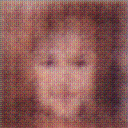
\includegraphics[width=150px]{500_fake_images/samples_5_400.png}%
\caption{A Black And White Photo Of A Man In A Mirror}%
\end{figure}

%
\end{document}